\documentclass [../article.tex]{subfiles}
\begin{document}
  \section{Patterns in Data}
  A real world application of Fourier Transform is when
  looking for patterns within what looks like useless or
  confusing data. In a blog, a person by the name Chad
  Orzel, decided to explain this exact use to those
  reading the blog. He gathered up data on the traffic the
  blog he writes in receives daily in the past one thousand
  and twenty-four days or about three years (to the power of
  two so it would work nicely with the transform).
  From the picture they show
  \begin{figure}[H]
    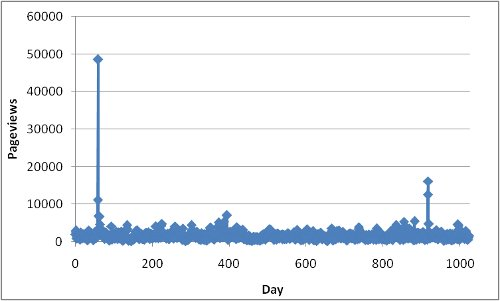
\includegraphics[width=\linewidth]{evar/1.jpg}
    \caption{Views Per Day.}
    \label{fig:views}
  \end{figure}
  you can not really discern anything special about this graph
  at all except for those two peaks where they had very popular
  blog posts at those times. With just looking at this graph
  alone and doing nothing else with it we do not learn much
  about this traffic. Now we apply fourier transform to this
  data set we get
  \begin{figure}[H]
    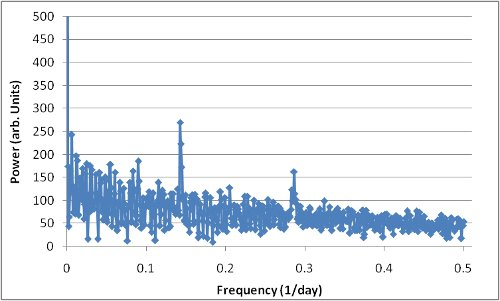
\includegraphics[width=\linewidth]{evar/2.jpg}
    \caption{View Frequency Spectrum.}
    \label{fig:viewfreq}
  \end{figure}
  This graph tells us how much on a certain sin wave they are
  using in order to re create the first graph shown. As you can
  see there are two relatively larger spikes in the graph
  excluding the one at “0” as that is another aspect of fourier
  transformation. These two spikes to tell us however that these
  two certain sin waves are occurring more often and such a
  possible pattern. In
  \begin{figure}[H]
    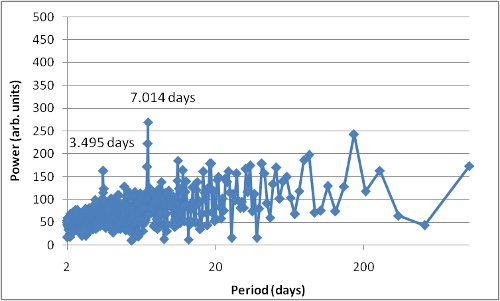
\includegraphics[width=\linewidth]{evar/3.jpg}
    \caption{View Period Strength.}
    \label{fig:viewperiods}
  \end{figure}
  the person plotted the function as one over the frequency as
  well as setting it up with a log scale. From this graph we see
  that through  fourier transformation we can notice that a very
  strong recurring pattern is occurring every week as well as a
  smaller one every half week.
  \begin{figure}[H]
    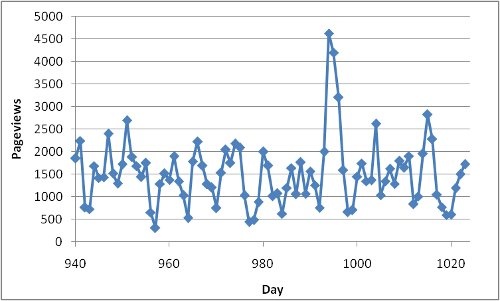
\includegraphics[width=\linewidth]{evar/4.jpg}
    \caption{Views Per Day Closeup}
    \label{fig:viewcloseup}
  \end{figure}
  Is a zoom in on our first graph showing this representation very
  well. Every seven days there is a strong dip downwards  which is
  why in the fourier transform graph there is a large appearance of
  a certain sin wave as well as the impact of the smaller wave every
  half week.

	In another example we are going to look at data over a certain
  amount of time, much like we did in the previous example. A
  person going by the name of Greg recorded the total number of
  user actions on their website. By looking at
  \begin{figure}[H]
    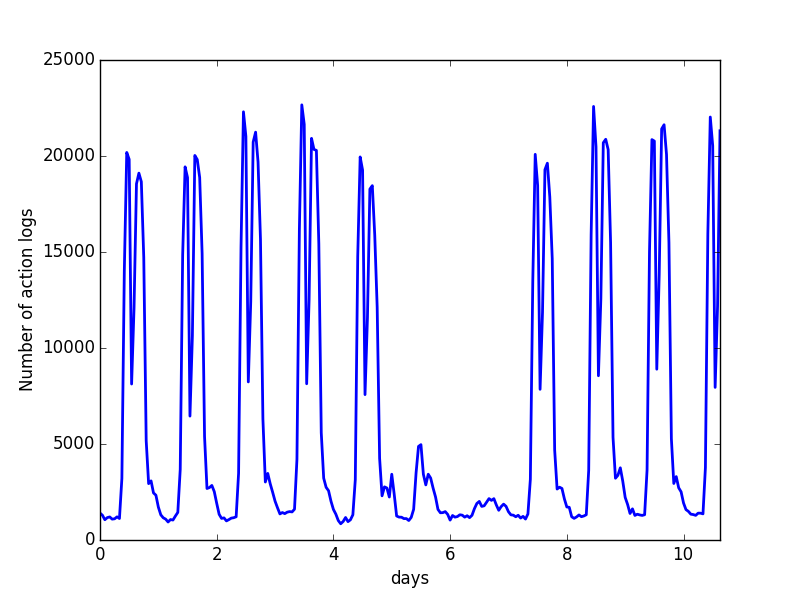
\includegraphics[width=\linewidth]{evar/5.png}
    \caption{User Actions.}
    \label{fig:useractions}
  \end{figure}
  you are easily able to identify a somewhat periodic pattern in
  the graph, but is there anything else that may be missing?
  Perhaps there is something we can not notice, so we use the
  fourier transform on the set. In
  \begin{figure}[H]
    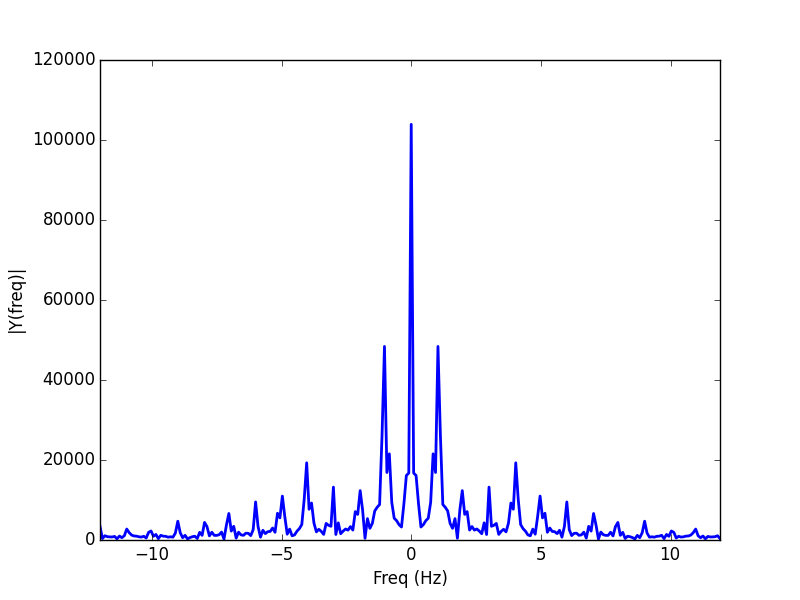
\includegraphics[width=\linewidth]{evar/6.png}
    \caption{User Action Spectrum.}
    \label{fig:actionspectrum}
  \end{figure}
  we notice that most of the actions on the site are using a low
  frequency sin wave. Now that the fourier transform in available
  we can directly compare the frequencies of the components to the
  original graph.
  \begin{figure}[H]
    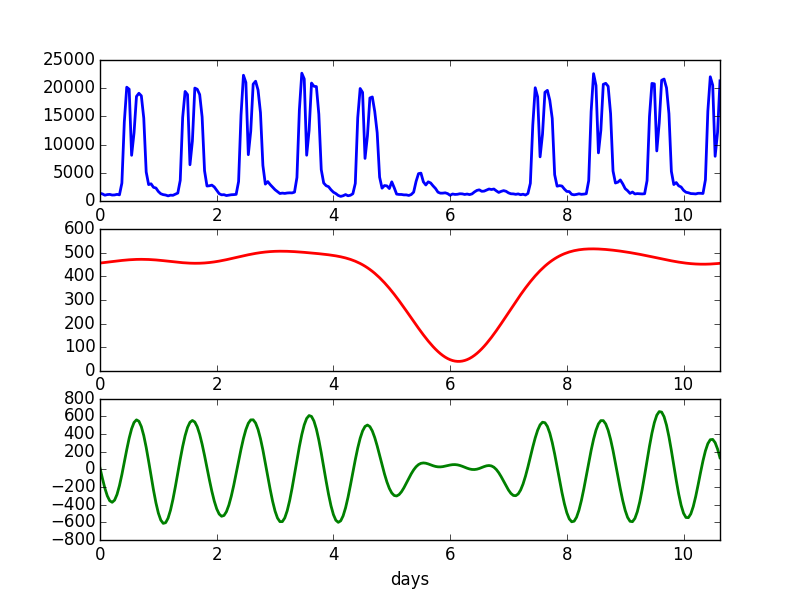
\includegraphics[width=\linewidth]{evar/7.png}
    \caption{I don't know.}
    \label{fig:idk}
  \end{figure}
  The second graph in the third image is the components of the
  transform with frequency less than |.46| and under that is
  components with frequency between |.46| and |1.40|.  The author
  notes that  the graph with the red line really shows how on
  weekends the amount of actions is extremely low and how the
  green graph shows how nice and fluid the dip is that represents
  when people are working and when they are not. We get a clear
  understanding of what exactly is going on if it it were possible
  to have access to more graph and at more frequencies we would be
  able to exactly replicate the original graph.

	With fourier transform we are able to see things we may not have
  been able to so in the past and even if we could allows us to
  understand it even more. With this technique people are able to
  base their programs and experiments with a much better evidence
  and data. It is also a really enjoyable thing to do in your free
  time.
\end{document}
